\documentclass[11pt,a4paper]{article}

\usepackage[T1]{fontenc}
\usepackage[utf8]{inputenc}
\usepackage[frenchb]{babel} % Global stuff set to french
\usepackage[margin=2.5cm]{geometry} % The margin of the page
%\usepackage{amsmath}  % to include math formulas
\usepackage{graphicx} % to include pictures
\usepackage[hidelinks]{hyperref} % To include hyperlinks in a PDF
\usepackage{fancyhdr} % to be able to make the page fancy looking
\usepackage{lastpage} % so latex knows what is the last page...
\usepackage{appendix} % To make appendixes
\usepackage{color} % For text colors
\usepackage{palatino} % Change font
%\usepackage{tabularx}
\usepackage{subcaption}
\usepackage{enumitem}
\usepackage{changepage}

%% Fancy layout
\pagestyle{fancy}
    \lhead{Projet d'année - Wizard Poker}
    \chead{}
    \rhead{Groupe 2}
    \lfoot{}
    \cfoot{}
    \rfoot{Page \thepage\ de \pageref{LastPage}}
\renewcommand{\headrulewidth}{0.4pt}
\renewcommand{\footrulewidth}{0.4pt}


%%% --- %%% --- DOCUMENT START --- %%% --- %%%
\begin{document}
    \begin{titlepage}

\topskip0pt
\begin{center}
    \vspace*{\fill}
        \hrule
        \vspace*{2pt}
        \hrule
        \vspace*{15pt}
        \textsc{\Huge{INFO-F106 : Projet d'année \\\vspace*{8pt} Rappport intermédiaire}}
        \vspace*{15pt}
        \hrule
        \vspace*{2pt}
        \hrule
  \vspace*{\fill}
\end{center}
\null
\vfill
  
\large{Mardi 16 décembre 2014} \hfill \large{Carlos Requena López - \emph{410031}}

\end{titlepage}
    \pagestyle{empty}
\tableofcontents
\newpage
 %%% Counting pages now %%%
\pagestyle{fancy}

\setcounter{page}{1}

\section{Introduction}
\label{sec:intro}

\subsection{But du projet}
\label{sec:but}

Dans le cadre du projet d'analyse et méthode et de système d'exploitation, il est demandé d'implémenter un jeu de carte en ligne basé sur une architecture client/serveur en C/C++.
\medbreak
Ce projet devra fournir un jeu de carte symétrique où deux joueurs pourront s'affronter et gagner des points pour un classement général. Chaque joueur disposera d'une collection de cartes à partir de laquelle il pourra construire des decks. Ces decks contiendront des cartes de type créature qui peuvent attaquer et des cartes de type sort qui lanceront des événements spéciaux.
\medbreak
Le projet requière la mise en place d'une architectures client/serveur avec le client qui sert principalement d'interface de jeu (graphique ou console) et les calculs qui seront effectué côté serveur. Il est donc important de développer un serveur robuste, efficace et rapide qui soit en mesure de gérer plusieures parties simultanément tout en fournissant des services tels que le classement général, un service de compte et de login ainsi qu'un service de messagerie instantané entre deux joueurs. Pour cela, nous seront ammené à développer une application capable de gérer un maximum de cas de figure pour garantir la continuité et la stabilité de ces différent services. La gestion d'erreurs devra être telle que cette erreur ne perturbera aucune autre partie ni aucun des autres services.
\medbreak
Le Wizard Poker sera disponible à n'importe quel joueurs enregistré pour jouer contre d'autres joueurs et essayer de gagner des places dans le classement générale. Il permetra aussi à de nouveaux joueurs de consulter ce classement et de s'enregistrer en tant que nouveau joueur. Dans ce cas, le joueur recevra ses premières cartes et sera invité à confectionner son premier deck avant d'affronter son premier adversaire.

% Texte (d’une demi-page approximativement) décrivant les tenants et
% aboutissants du projet, et énumérant les différents types de
% personnes qui vont bénéficier de la réalisation du projet.

\subsection{Glossaire}
\label{sec:glo}

% Définition des termes, des acronymes et des abréviations utilisés
% dans le présent document.

\begin{itemize}
  \item \textbf{Deck:} Collection de 20 cartes qui...
  \item \textbf{Collection:} Ensemble de cartes
  \item \textbf{tchat:} Messagerie instantanée permettant à 2 personnes de s'échanger des messages écrit
\end{itemize}

\subsection{Historique du document}
\label{sec:hist}

% Tableau reprenant tous les changements effectués sur le
% document. Chaque ligne de celui-ci contiendra les champs suivants :
% numéro de version, auteur et date de la modification, description
% des changements. Le tableau sera trié de manière décroissante sur le
% numéro de version.

% Example de versioning:


    % 0 for alpha (status)
    % 1 for beta (status)
    % 2 for release candidate
    % 3 for (final) release


\begin{table}[h]
  \centering
  \begin{tabular}[ht]{|l|l|l|p{18em}|}
    \hline

    \textbf{Version}
    & \textbf{Auteur}
    & \textbf{Date modification}
    & \textbf{Description des changements}\\ \hline \hline
    NEXT &  &  &  \\ \hline
    NEXT &  &  &  \\ \hline
    v0.3 & Rémy et Lucie  & 11/12/15 16h20 & Ajout de diagrammes, ajout de ``Exigences du domaine'' \\ \hline
    v0.2 & Amin Abdelkefi & 10/12/15 23:45 & Ajout de la partie ``Exigences fonctionnelles''\\ \hline
    v0.1 & Jonas et Raphaël & 10/12/15 13:28 & Ajout de la partie ``But du projet''\\ \hline
    v0.0 & Carlos Requena & 26/11/15 22:30 & Mis en place. Diagrammes realisés en groupe le 25/11/15 ajoutés\\ \hline
  \end{tabular}
  \caption{Changements document}
  \label{tab:hist}
\end{table}

\section{Besoins de l'utilisateur}
\label{sec:besoins}

% Cette deuxième section reprend les services que le système doit
% fournir aux utilisateurs, ainsi que les contraintes de
% fonctionnement du système. Elle doit être complète et consistante,
% et il faut qu’elle soit rédigée dans un langage spécialement
% compréhensible pour le client, c’est-à-dire en évitant entre autres
% tout terme ou détail techniques.

\subsection{Exigences fonctionnelles}
\label{sec:exi-fonc}
  \begin{figure}[ht]
    \centering
    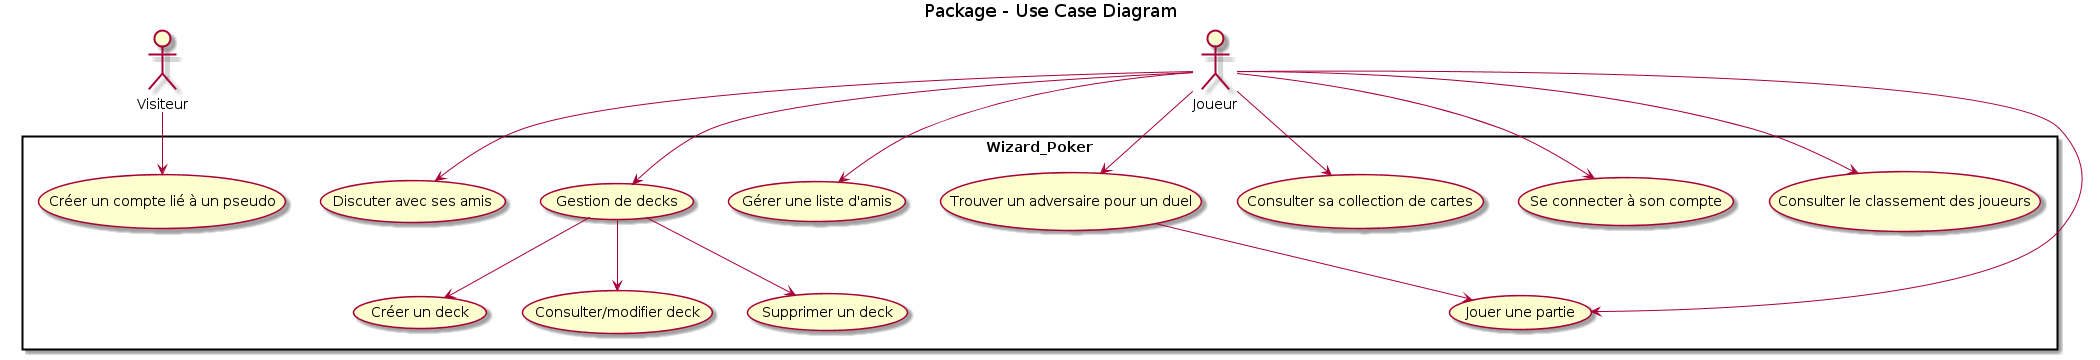
\includegraphics[width=1\textwidth]{uml_files/UseCaseDiagram.png}
    \caption{\label{fig:usecase} Use Case Diagram du jeu en question}
  \end{figure}
  
  \subsubsection{Créer un compte lié à un pseudo}
    Tout visiteur se verra offerte l'opportunité de se créer un compte lié à un pseudo (si ce dernier est disponible) afin de pouvoir profiter pleinement du jeu.

  \subsubsection{Se connecter à son compte}
    Le joueur devra se connecter à son compte s'il souhaite effectuer les différentes actions répertoriées ci-dessous.

  \subsubsection{Consulter sa collection de cartes}
    Le joueur peut consulter l'ensemble des cartes présentes dans sa collection. Pour cela, il devra au préalable s'être connecté.

  \subsubsection{Gestion de decks}
    Un deck est un ensemble de cartes qui sera utilisé par le joueur lors d'un duel. Plusieurs actions peuvent être effectuées sur les decks telle qu'en supprimer un ou plusieurs, les consulter, les modifier ou tout simplement en créer un nouveau.

  \subsubsection{Gérer une liste d'amis}
    Chaque joueur aura une liste d'amis avec lesquels il pourra interagir s'il le souhaite. Il pourra aussi ajouter un amis à sa liste ou en supprimer.

  \subsubsection{Discuter avec ses amis}
    Le joueur pourra, à tout moment, parler avec un ou plusieurs de ses amis actuellement connectés. Pour cela, un tchat sera mis à disposition du joueur.  Le joueur pourra donc communiquer avec ses amis par message à tout moment.

  \subsubsection{Proposer une partie à un ami}
    Si le joueur le souhaite, il peut proposer une partie avec un de ses amis connectés si ce dernier accepte cette demande.

  \subsubsection{Trouver un adversaire pour un duel}
    Lorsqu'un joueur voudra lancer une partie, le jeu trouvera automatiquement un adversaire dans la liste des personnes connectées.  Le choix est totalement aléatoire.

  \subsubsection{Consulter le classement}
    Le classement va permettre de classer les joueurs en fonction de leur nombre de victoires et de leurs défaites. Ce classement se basera donc sur le ratio victoire/défaites. 
 

% Ce type d’exigences sera décrit en utilisant des diagrammes use case
% et en fournissant une description pour chacun d’entre eux (comme vu
% au cours théorique et aux exercices).

\subsection{Exigences non fonctionnelles}
\label{sec:exi-nonfonc}

  % Question: ne nous a t'on pas dit que cela devait être secondaire ? :/
  % J'ai l'impression qu'on s'engage à faire beaucoup de choses ici mais en même temps je vois pas quoi mettre d'autre...
  \subsubsection{Ergonomie}
    Créer un jeu qui sera simple d'utilisation et facilement compréhensible pour un utilisateur n'ayant jamais joué à un jeu de ce genre.\\
    Pour cela, on peut rendre l'interface intuitive à l'aide de ``boutons'' décrivant exactement leurs utilités ou encore à l'aide d'un rapide tutoriel après la création du compte expliquant les différentes caractéristiques du jeu.

  \subsubsection{Design}
    Le design est l'apparence qu'aura l'interface graphique. Comme pour le point précédent, une belle interface va permettre à l'utilisateur de facilement voir les différentes possibilités offertes par le jeu en plus d'apprécier l’esthétique.\\
    Le design est un ``domaine'' (vague) c'est-à-dire qu'il définit l'apparence du jeu mais aussi les différents sons et/ou musiques.

  \subsubsection{S'amuser}
    Qu'est-ce qu'un bon jeu?\\
    Un bon jeu est un jeu attractif, beau, facile à comprendre mais avant tout, un bon jeu est jeu où l'on s'amuse. Notre principal objectif sera de réaliser ce jeu et de permettre à tout les joueurs de s'amuser. (?????? A changer si vous le souhaitez)


\subsection{Exigences de domaine}
\label{sec:exi-dom}

  Le domaine du jeux vidéo laisse beaucoup de liberté.  En effet, chaque créateur essaye de créé son univers, de développer son concept.  Cependant, tous les jeux doivent permettre à leur utilisateur de trouver du plaisir ou une certaines forme de satisfaction.  Il faut également éviter que le joueur soit interrompu durant sa partie.  Les exigences du domaine ne sont donc pas nombreuses mais compliqué à satisfaire complètement.\\
  Pour résumé, un utilisateur attend de l'amusement et une stabilité acceptable (voir infaillible coté serveur).  Nous nous concentrerons dans un premier temps (dans le cadre de ce projet) à ce deuxième point.
  % TO DO: à compléter/modifier
  
  
\section{Besoins du système}
\label{sec:besoins-sys}

% Cette troisième section décrit en détail les fonctionnalités du
% système (à partir de celles décrites à la section précédente), sans
% aborder (dans la mesure du possible) *comment* elles doivent être
% réalisées.

\subsection{Exigences fonctionnelles}
\label{sec:exi-fonc-sys}

% Ce type d’exigences sera décrit en utilisant des diagrammes use
% case et en fournissant une description *plus détaillée* pour
% chacun d’entre eux (comme vu au cours théorique et aux exercices).

Sequence diagram pour interaction??

Le système doit interagir avec l'utilisateur, et lui proposer certaines actions, comme commencer un duel, gérer ses decks, consulter le classement des joueurs, etc.

Pour les nouveaux joueurs, l'application doit offrir la possibilité de s'enregistrer, avec un pseudonyme et un mot de passe.


\subsection{Exigences non fonctionnelles}
\label{sec:exi-nonfonc-sys}

Les exigences non fonctionnelles décrivent le comportement de l'application.

Le système doit être tout d'abord robuste et stable, c'est-à-dire gérer les erreurs et éviter les crashs et les déconnexions... Il doit par ailleurs être agréable d'utilisation pour l'utilisateur (ergonomie et esthétique/design) et garantir que celui-ci ne puisse pas tricher pendant une partie.

Donc en résumé, robuste, stable, sûr, et excessivement amusant. Des heures de franche rigolade, en toute sécurité, sont assurées à tout utilisateur du jeu.

\subsection{Design et fonctionnement du systeme}
\label{sec:design}

% Cette partie sera décrite à l’aide des différents diagrammes UML
% vus au cours théorique et aux exercices.

% Peut être le supprimer vu qu'il est déjà  plus haut
\begin{figure}[ht]
  \centering
  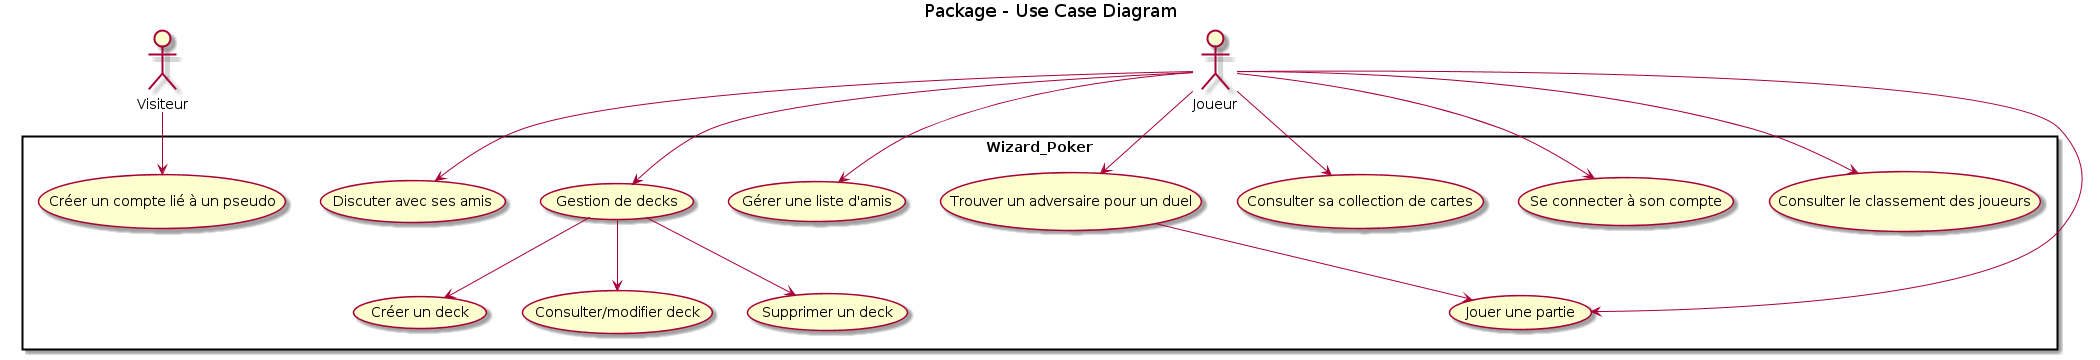
\includegraphics[width=1\textwidth]{uml_files/UseCaseDiagram.png}
  \caption{\label{fig:usecase} Use Case Diagram du jeu en question}
\end{figure}

% A voir si on ne remplace pas cette image par la suivante
\begin{figure}[ht]
  \centering
  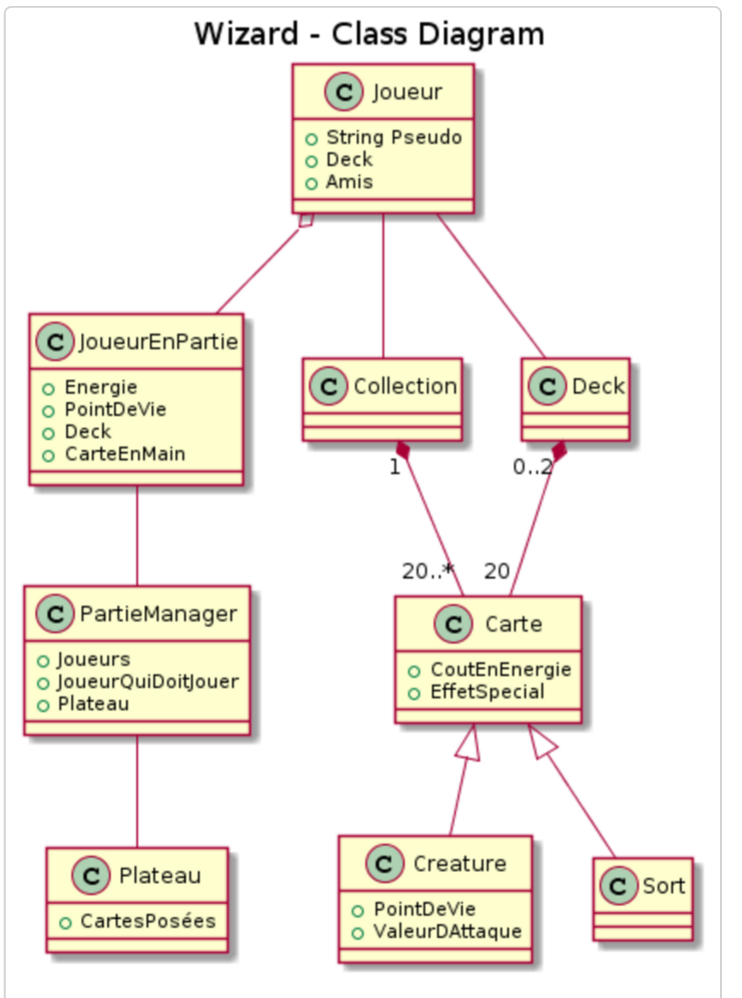
\includegraphics[width=1\textwidth]{uml_files/ClassDiagram.png}
  \caption{\label{fig:class} Diagramme des classes}
\end{figure}

\begin{figure}[ht]
  \centering
  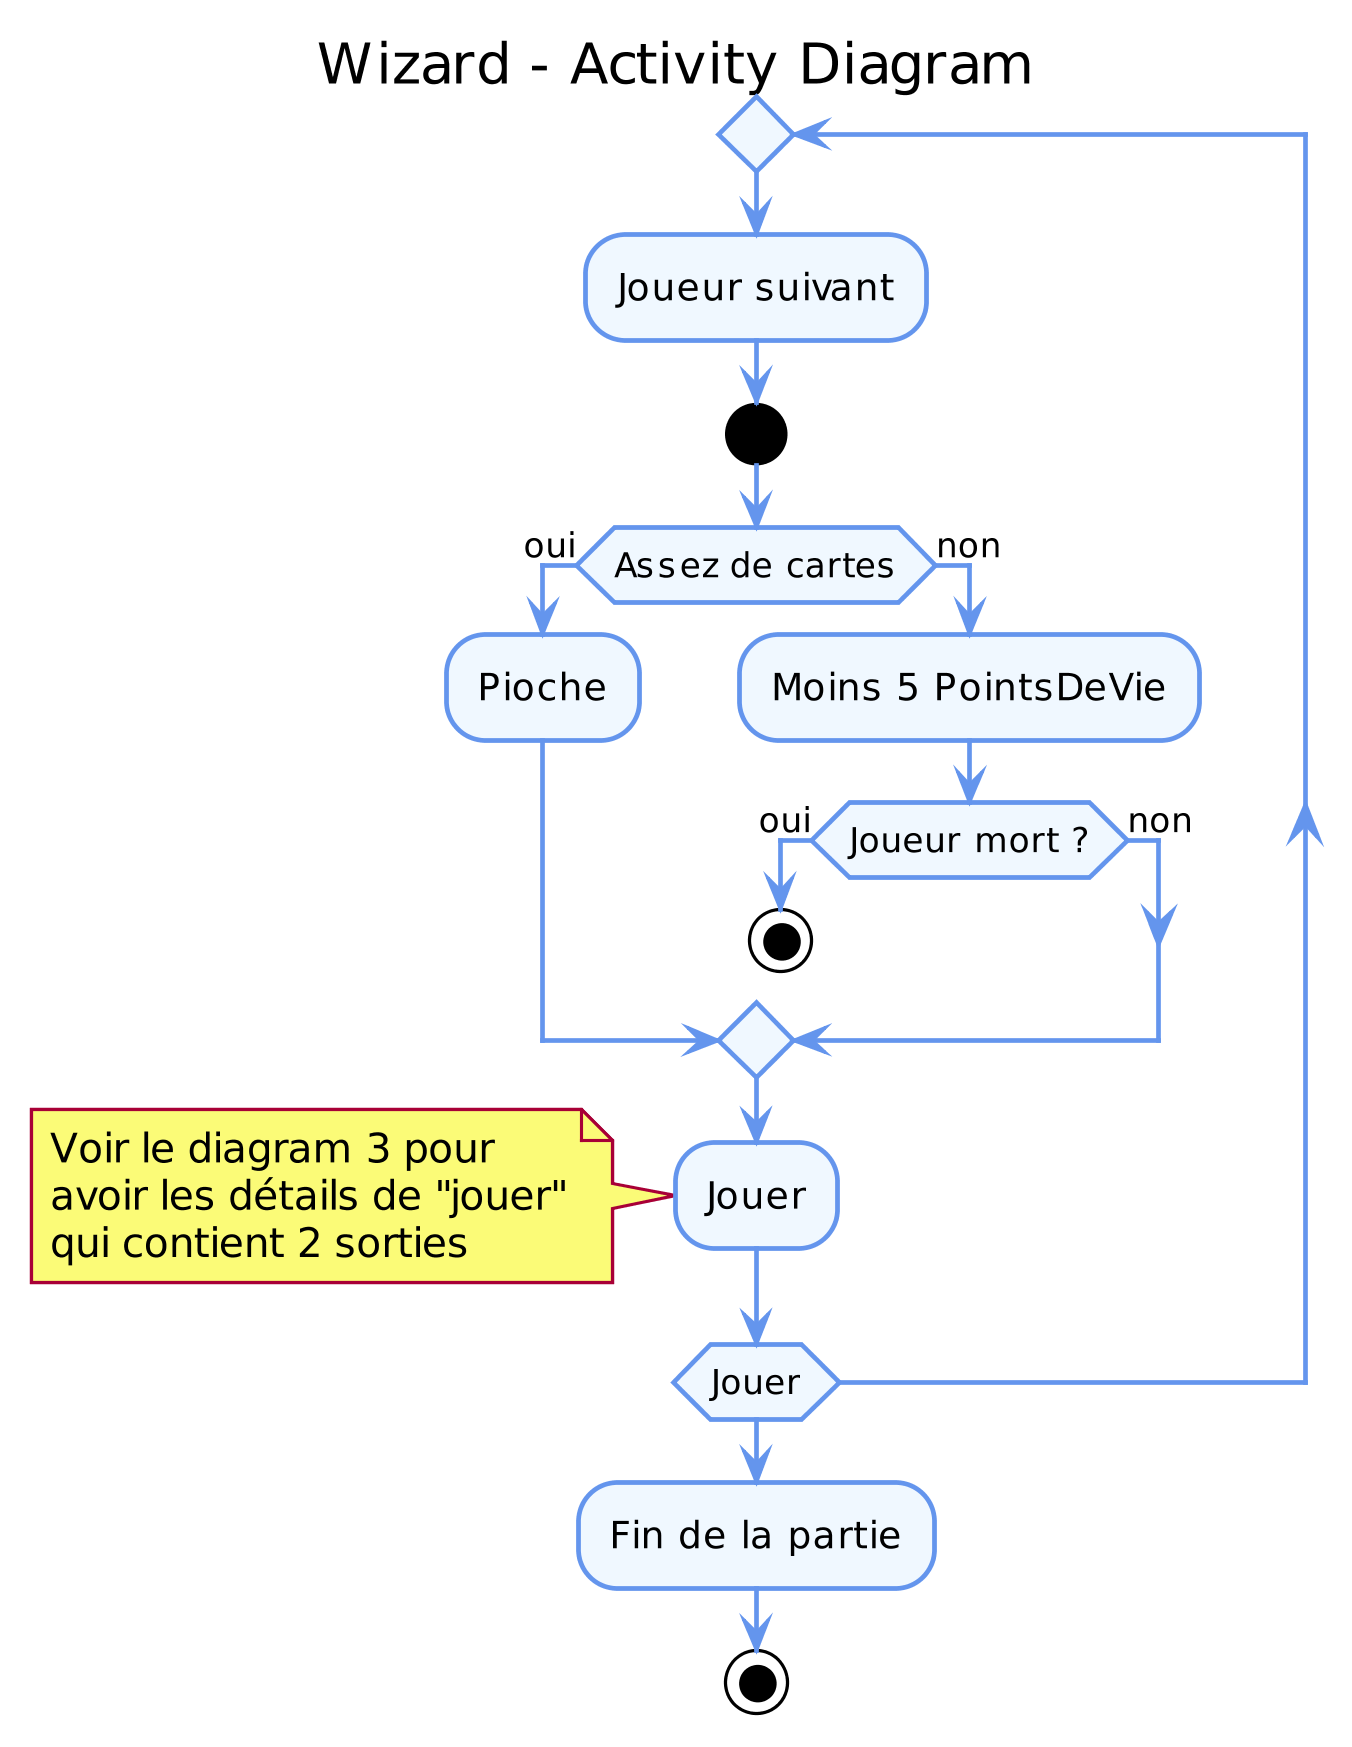
\includegraphics[width=1\textwidth]{uml_files/ActivityDiagram.png}
  \caption{\label{fig:class} Diagramme d'activité}
\end{figure}

\begin{figure}[ht]
  \centering
  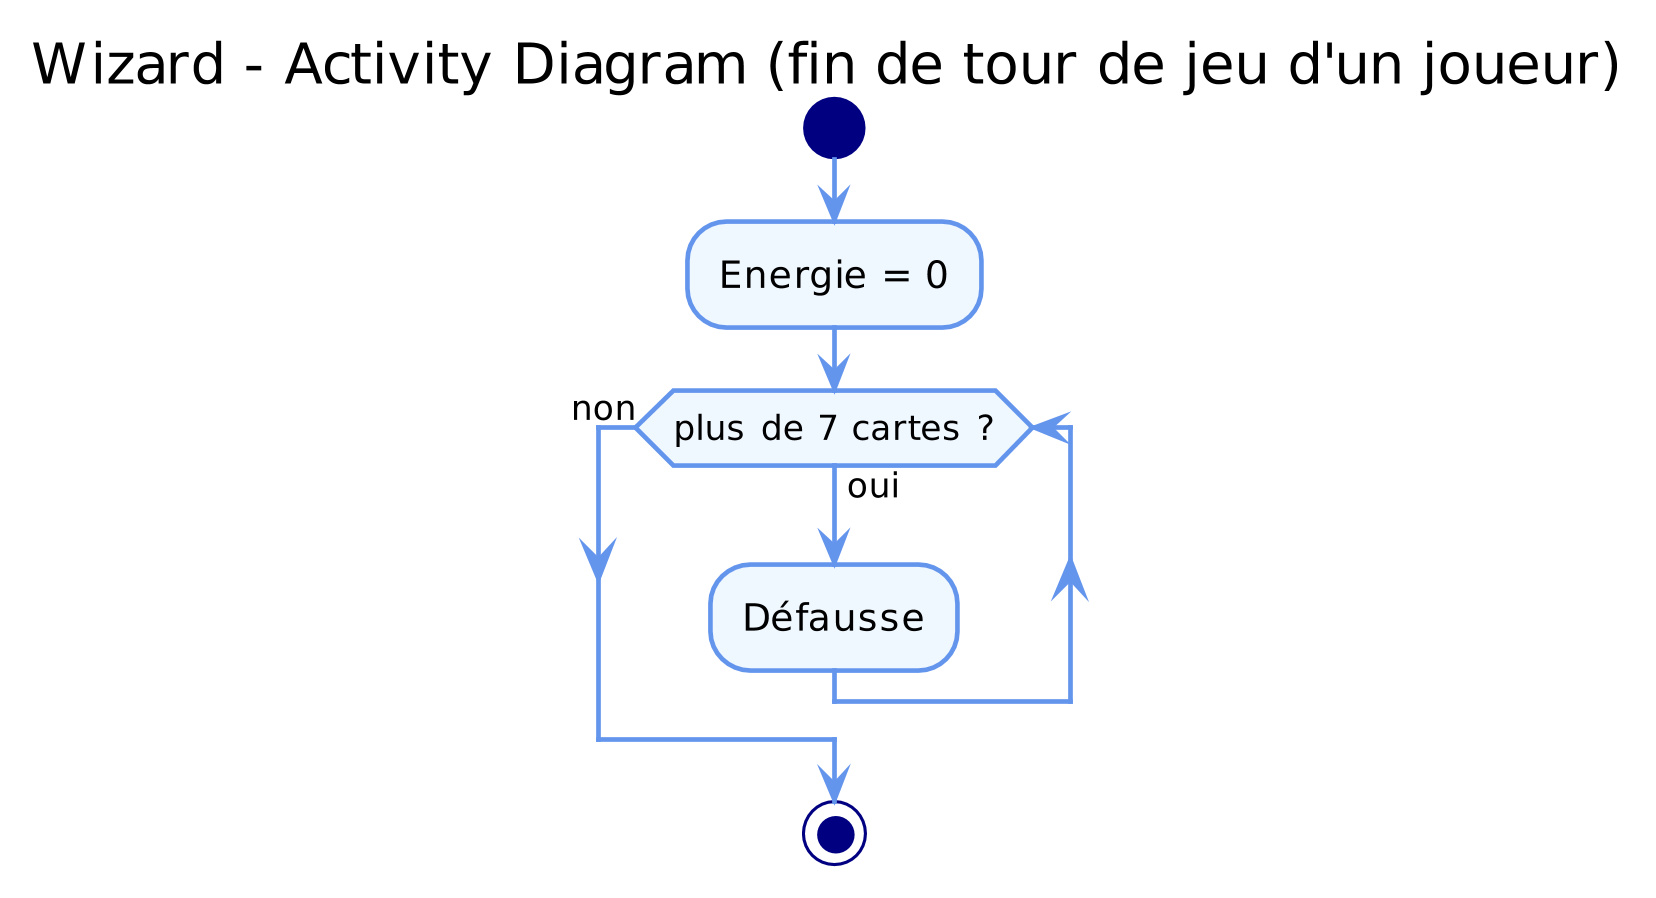
\includegraphics[width=1\textwidth]{uml_files/ActivityDiagram2.png}
  \caption{\label{fig:class} Diagramme d'activité 2}
\end{figure}

\begin{figure}[ht]
  \centering
  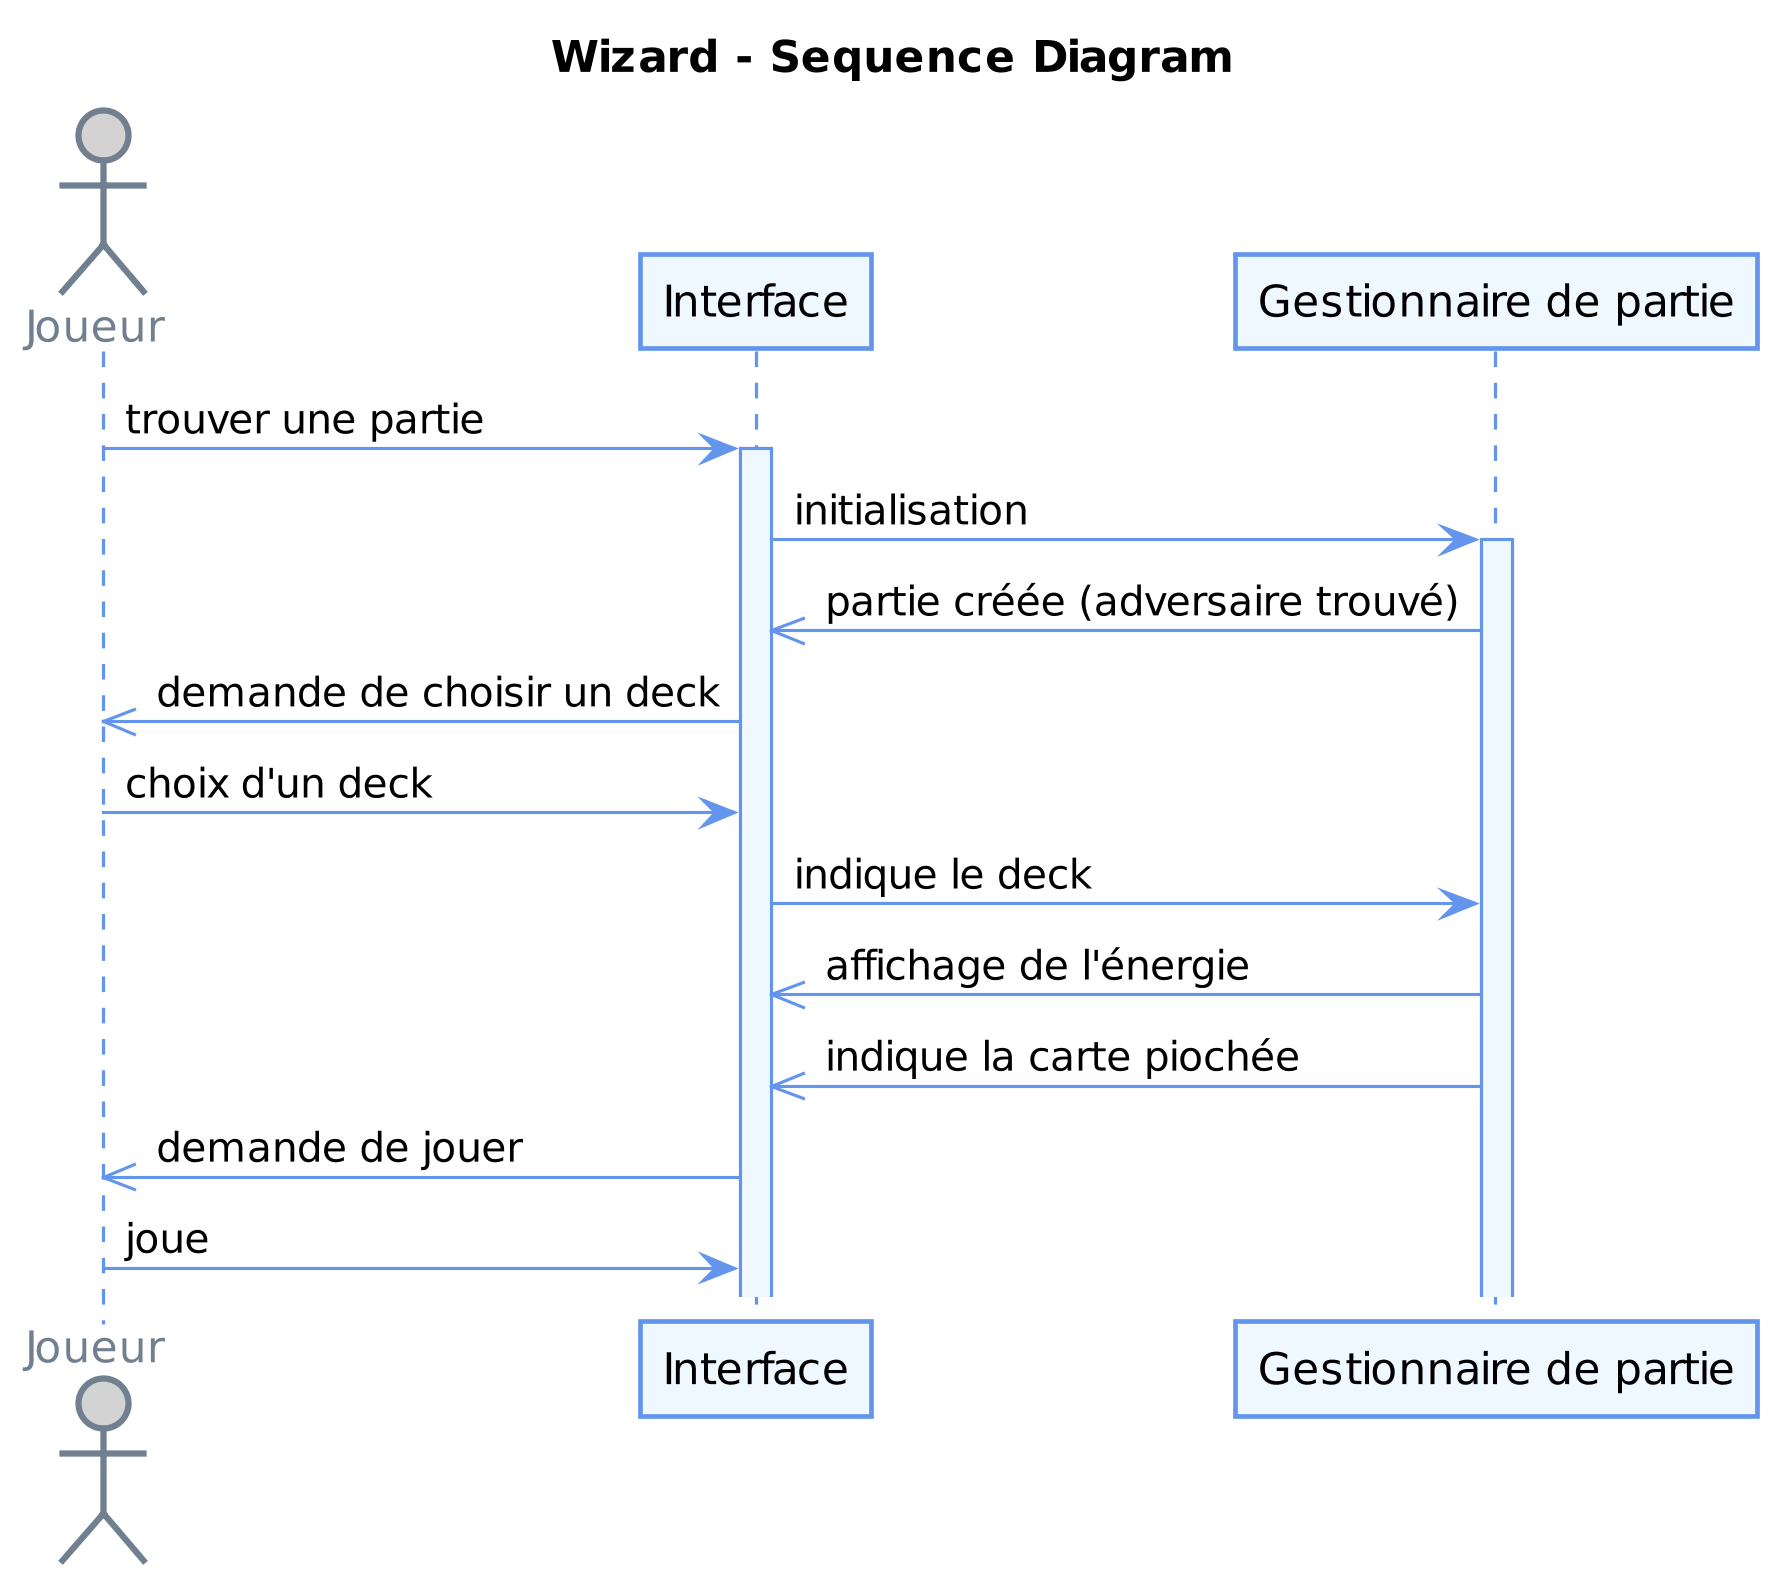
\includegraphics[width=1\textwidth]{uml_files/SequenceDiagram.png}
  \caption{\label{fig:class} Diagramme de séquence}
\end{figure}

\appendix

\section{Index des termes utilisés}
\label{sec:index}

\end{document}
